Медленное многообразие для системы (\ref{fullt}) представляет собой множество:
$$M_0 = \{(x, y, \lambda, \Lambda): \Lambda = 0, u(x,y) \sin \lambda = v(x,y) \cos \lambda \}.$$

Условие $U \sin \lambda = V \cos \lambda$ эквивалентно $\lambda = \arctan(V/U) + \pi k$, $k \in \mathbb{Z}$. Для устранения разрывов при $U = 0$ вводятся две непрерывные функции $\lambda_{\pm}: \mathbb{R}^2 \setminus \{U=V=0\} \to S^1$, отличающиеся на $\pi$:
$$
\lambda_{+}(x,y) \equiv \begin{cases} 
        \arctan \frac{V}{U},        &  U>0, V > 0, \\
        \arctan \frac{V}{U} + \pi,  &  U<0, \\
        \arctan \frac{V}{U} + 2\pi, &  U>0, V<0,
       \end{cases}
\quad
\lambda_{-}(x,y) \equiv \begin{cases} 
        \arctan \frac{V}{U} + \pi,  &  U>0, V > 0, \\
        \arctan \frac{V}{U} + 2\pi, &  U<0, \\
        \arctan \frac{V}{U} + 3\pi, &  U>0, V<0.
       \end{cases}
$$

В особых точках, где $U = V = 0$, решение дает две окружности:
$$y=0,\quad x=x_b^{\pm}\equiv\frac{-e_JD \pm e_J \sqrt{D^2-4EC}}{2C},\quad \Lambda=0,\quad \lambda\in S^1.$$

Локально вблизи этих точек медленное многообразие имеет структуру винтовой поверхности, описываемой уравнением $\tan\lambda = y/(x-x_b^{\pm})$.

\begin{figure}[H]
\centering
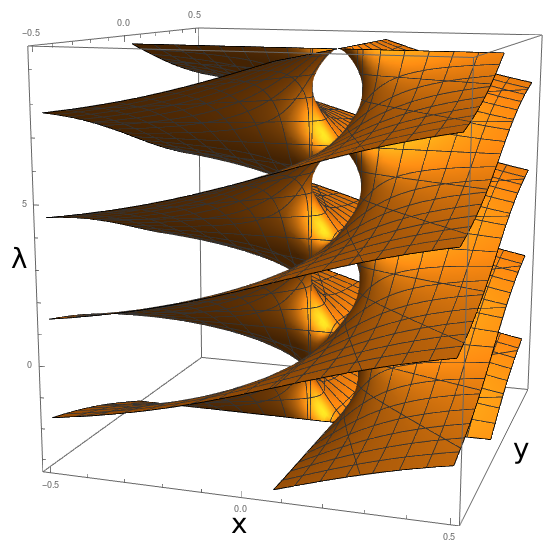
\includegraphics[scale=0.55]{../img/MM.png}
\caption{}
\end{figure}

Таким образом, медленное многообразие представляет собой два листа $M_{0,\pm}$, соединенных двумя перемычками $M_{0,b}^{\pm}$:

\begin{align*}
M_0 &= M_{0,+} \cup M_{0,-} \cup M_{0,b}^{+} \cup M_{0,b}^{-}, \\
M_{0,\pm} &= \{ \lambda = \lambda_{\pm}(x,y), \Lambda = 0, (x,y) \in \mathbb{R}^2 \setminus \{U=V=0\} \}, \\
M_{0,b}^{\pm} &= \{ y=0, x=x_b^{\pm}, \Lambda=0, \lambda\in S^1 \}.
\end{align*}

Листы $M_{0,\pm}$ гомеоморфны плоскости с двумя выколотыми точками, а перемычки $M_{0,b}^{\pm}$ - окружностям.